
\section{Numerical setup} \label{sec:NumSetUp}
The objective of the present simulation setup is to obtain a TBL developing under a moderate APG over a long region of near-equilibrium flow from low to high Reynolds numbers. To achieve a high-Reynolds-number simulation starting from a laminar flow we have taken as a reference the ZPG LES simulation by \cite{E-AmorZPG} based on \cite{Schlatter_etAl_LES_2010}, which on itself was validated using DNS by \cite{schlatter_orlu_2010}. The box size in the streamwise direction ($L_x$) was chosen to be identical to that of the ZPG simulation. The effect of an APG will increase the growth rate of the boundary layer together with the size of the energetic scales, and in order to account for this we increased the box size in the wall-normal ($L_y$) and spanwise directions ($L_z$) with respect to the values used by \cite{E-AmorZPG}, as can be observed in table \ref{tab:param}. Since the code used for the simulation, SIMSON \citep{simson_techrep}, uses Fourier modes in the streamwise direction, all the flow that has exited the domain through the top boundary due to the growth of the boundary layer, needs to enter again into the domain at the end of the box through a fringe region. 
The fringe length in the APG case will have to be longer than in the ZPG configuration, since a larger amount of flow leaves the domain in the former case and it will need to return through a negative wall-normal velocity component $V$, which will increase the Courant--Friedrichs--Lewy (CFL) number. The time step of the simulation was kept constant in order to perform Fourier analysis of the temporal series of the velocity components. Therefore, in order to have a constant time step that would not be too low and maintain a stable CFL, the fringe length had to be increased so the maximum $V$ was reduced in that region. It is important to mention that the CFL also depends on the spatial discretization, and since SIMSON uses Chebyshev polynomials in the wall-normal direction $y$, the wall-normal grid spacing ($\Delta y$) at the top boundary is too fine, if this spacing could be increased, then the CFL number would be reduced and it would be possible to use a shorter fringe with a higher $V$.

\subsection{Parameters of the simulation} \label{subsec:Param_sim}
The streamwise, wall-normal and spanwise coordinates $(x,y,z)$ and other lengths or distances are non-dimensionalized with the reference length $\delta^*_0$ (which is the displacement thickness of the inflow laminar boundary layer). In some parts of the text $\delta^*_0$ is not written for the sake of simplicity. That is also the case for the velocities, which are non-dimensionalized with the inflow free stream velocity $U_{\rm ref}$.
For all of the simulations in table \ref{tab:param} the same code (SIMSON) was employed, and the well-resolved LES is based on the same sub-grid-scale (SGS) model, ADM-RT, which stands for approximate deconvolution relaxation-term \citep{Schlatter_2004}, as discussed in more detail in appendix \hyperlink{AppB}{B}. In the present simulation, denoted by b1.4, we have used a new feature in the code: the implementation of message-passing interface (MPI) communication in single precision. In this version of the code, all the computations continue to be in double precision, but the time spent in communication between processors has been reduced by casting the data into single precision and reducing by half the amount of data to communicate. 

After selecting the box size we proceed to run the simulation with ZPG boundary conditions (BC) at a low resolution. The initial conditions and inflow profile are given by a laminar Blasius boundary layer with a displacement thickness $\delta^*_0$ such that $Re_{\delta_0^*}=450$. The flow is tripped to turbulence close to the inlet at $x/\delta^*_0=10$ using a volume forcing \citep{schlatter_orlu_2012}, which is the same method as in the other databases, and with this configuration we expect the transition to turbulence to be over at $Re_{\theta}\approx 600$ \citep{E-AmorZPG, schlatter_orlu_2012}. The TBL will develop to high Reynolds numbers over a long computational domain in a similar way as it is done in a wind-tunnel experiment. This is different from setting up an auxiliary ZPG simulation and using a recycle plane for the inflow as used in \cite{Kitsios2016, Kitsios2017, Gungor_DNS_2017}, since the APG BCs downstream would affect the initial ZPG, as can be seen in figure \ref{fig:U_BCs}. At the end of the domain a fringe region \citep{SIMSON_fringe} reduces the turbulence and yields the same laminar flow as the inflow in order to obtain the periodicity required by the Fourier discretization. 
One flow-through is defined as the time required by the flow to pass through the domain once; here the mean streamwise velocity is of the order of the unity, so we will approximate the time required by the flow to cover a distance $L_x$ to be equal to that distance. When the flow is fully turbulent after $\sim3$ flow-through times we proceeded to progressively change the APG BC to the desired distribution. In the final APG configuration, a fringe length of $1500 \delta^*_0$ is needed to keep the simulation stable.
The simulation was run for enough time for the statistics to converge \citep{vinuesa2016_mec} after excluding the initial transients due to the change of resolution. 
The statistics were averaged for over 8 and 4 eddy-turnover times (ETT) at the middle and the end of the region of interest respectively (note that the region of interest ends before the fringe). In APG TBLs the eddy-turnover time varies significantly with $x$, and it is calculated as: $ {\rm ETT}(x) = \Delta T  u_{\tau}(x) / \delta_{99}(x)$, with $\Delta T$ being the period of time used for averaging and $u_{\tau}(x)=\sqrt{(\tau_w / \rho)}$ the friction velocity.
We also collected time series containing 36,000 samples over the same period. 
The time step of the simulation is held constant at $\Delta t_{\rm step}=0.25$, which ensures that in viscous units the time step along the domain is $\Delta t_{\rm step}^+ \leq 0.35$. The statistics were sampled every 4 time steps in the region of interest, which corresponds to $\Delta t_{\rm stat}^+ \leq 0.5$.
The viscous scaling (denoted by the superscript `+') for velocity, length and time scales is:  $u_{\tau}$, $l_{\tau}=\nu/u_{\tau}$ and $t_{\tau}=l_{\tau}/u_{\tau}$.

In table \ref{tab:param} we show the box size, the collocation points using the 3/2 factor for de-aliasing ($m_x, m_y, m_z$) and the resolution of the various simulations. With the previous parameters we obtain the streamwise and spanwise resolution in viscous units ($\Delta x^+ , \Delta z^+$). The maximum separation of grid points in the wall-normal direction inside the boundary layer is shown in viscous units as $\Delta y_{\rm max}^+$, and it occurs close to the boundary-layer edge at the highest Reynolds numbers. In the new simulation b1.4, for $Re_{\tau}=500$, the number of grid points below $y^+=10$ is 6, below $y^+=1$ we have 2 and the distance of the first grid point from the wall is $\Delta y_w^+=0.3$. Since the viscous length scale $l_{\tau}$ increases with the streamwise position, the resolution in viscous units close to the wall will be better at higher Reynolds numbers: for $Re_{\tau}=800$ we have 7 grid points below $y^+=10$, 3 grid points below $y^+=1$ and $\Delta y_w^+=0.2$.
The color code that will be used along this work is shown in table \ref{tab:param}.

\begin{table}
  \begin{center}
  \fontsize{8.0pt}{10.25pt}\selectfont
  \addtolength{\tabcolsep}{-2pt}
\def~{\hphantom{0}}
    \begin{tabular}{ l r  r  r  r  r  r  r  r  r  r  r r}
    Case  & $L_x/\delta_0^*$ & $L_y/\delta_0^*$ & $L_z/\delta_0^*$ & $m_{x}$ & $m_{y}$ & $m_{z}$ & $\Delta x^{+}$ & $\Delta y_{\rm max}^{+}$ & $\Delta z^{+}$ & Colour & Reference \\[3pt]
    
    b1             &    3000   &   140   &    250  &    3072 &     301 &     576 &   21.8    & 8.4 &   9.7  & \redline     & Bobke (\citeyear{bobke2017}) \\
    b2             &    3000   &   180   &    320  &    3072 &     361 &     768 &   21.6    & 7.9 &   9.2  & \greenline   & Bobke (\citeyear{bobke2017}) \\
    m16            &    3000   &   180   &    220  &    3072 &     361 &     576 &   21.2    & 7.7 &   8.3  & \blueline    & Bobke (\citeyear{Bobke_2016}) \\

    ZPG            &   13500   &   400   &    540  &   13824 &     513 &    1152 &   22.6    & 19.6 &  10.9  & \blackline  & Eitel-Amor (\citeyear{E-AmorZPG}) \\
    b1.4           &   13500   &   800   &   1080  &   13824 &     301 &    1920 &   21.7    & 30.1 &  12.5  & \orangeline & Present study \\

    \end{tabular}
  \caption{Parameters of the simulations used in this paper. The inlet displacement thickness $\delta_0^*$ corresponds to the displacement thickness of a laminar flow for a Reynolds number $Re_{\delta_0^*}=450$. The box size is $(L_x/\delta_0^*, L_y/\delta_0^* , L_z/\delta_0^*)$  and $(m_x, m_y, m_z)$ are the number of collocation points including the $3/2$ factor for de-aliasing in the Fourier directions ($x$ and $z$). The spatial resolution in viscous units $(^+)$ of the streamwise and spanwise directions $\Delta x^{+}, \Delta z^{+}$, has been calculated using $(m_x, m_z)$ at the position $x/\delta_0^*=250$, which corresponds to a friction Reynolds number $Re_{\tau}\approx 210$ for all the simulations. The maximum viscous distance between grid points in the wall-normal direction inside the boundary layer is observed close to the boundary-layer edge and for the highest Reynolds number of each simulation. }
  \label{tab:param}
  \end{center}
\end{table}

The Reynolds-number and pressure-gradient ranges are shown in table \ref{tab:ROI},together with the region of interest (ROI) for each simulation. 
The ROI in the APG cases starts at the point where the maximum $\beta$ is achieved, while in the ZPG TBL, the starting point is taken at $Re_{\tau}=500$, which approximately corresponds to $Re_{\theta}\approx 1500$, where according to \cite{E-AmorZPG, schlatter_orlu_2012} the flow is independent of the inflow conditions and the tripping.
The last point of the ROI was chosen as the position where the skin-friction coefficient exhibits a clear tendency upwards due to the effects of the fringe; note that the large scales have not been affected yet.
In the ROI we observe a slowly-decaying positive $\beta$, where $\overline{\beta}$ is the average $\beta$ along the ROI. Note that this is not the accumulated $\overline{\beta}$ defined by \cite{Vinuesa_2017}, but a simple average instead. The standard deviation is $\sigma({\beta})$ and these quantities, together with the defect shape factor  $G=(H_{12}-1)/(H_{12}\sqrt{c_f/2})$, are given in table \ref{tab:ROI}. Note that $H_{12}$ and $c_f$ are the shape factor and the skin-friction coefficient, respectively. In the ROI of the b1.4 case, $G$ lies between 10.5 and 11.6, which is in agreement with the results reported by \cite{bobke2017}: 9.8 and 12.1 for the b1 and b2 cases, respectively.
\begin{table}
  \begin{center}
    \fontsize{8.0pt}{10.25pt}\selectfont
  \addtolength{\tabcolsep}{-2pt}
\def~{\hphantom{0}}
    \begin{tabular}{ l c  c  c  c  c  c c c}
    Case  & Range of $x/\delta_0^*$ & Range of $Re_{\tau}$ &  Range of $Re_{\theta}$ & Range of $\beta$ & $\overline{\beta}$ & $\sigma({\beta}) / \overline{\beta}$ & $G$ \\[3pt]
    
    b1             &     718 --  2101   &  350 -- 750   &  1320 -- 3080  & 1.12 -- 0.85 & 0.99 &  0.08 &    9.8 -- 10   \\
    b2             &    1148 --  2001   &  480 -- 730   &  2260 -- 3530  & 2.19 -- 1.86 & 2.06 &  0.04 &   12.1 -- 12.3 \\
    m16            &     823 --  2001   &  370 -- 740   &  1790 -- 3650  &  2.8 -- 1.9  & 2.42 &  0.11 &   12.5 -- 13.5 \\

    ZPG            &    1251 -- 11666   &  500 -- 2500  &  1430 -- 8200  &  $\simeq 0$  & $\simeq 0$ & $\simeq 0$ &   7.1 -- 7.2 \\
    b1.4           &    2455 --  8117   &  800 -- 1900  &  3700 -- 8700  & 1.65 -- 1.20 & 1.41 &  0.10 &   10.5 -- 11.6  \\
    \end{tabular}
  \caption{ Flow characteristics in the ROI for the various cases.}
  \label{tab:ROI}
  \end{center}
\end{table}


\subsection{Boundary conditions} \label{subsec:BC}

These simulations are statistically homogeneous in the spanwise direction $z$, therefore, they are statistically two-dimensional in the streamwise and wall-normal directions, and have periodic boundary conditions in the streamwise and spanwise directions. 
Since no cross-flow is present in the spanwise direction the only boundary condition (BC) is imposed by the periodicity. In the streamwise direction, the periodicity forces the outflow to be the same as the inflow, and this is achieved through a fringe region as mentioned above. 
The inflow is given by a Blasius boundary layer at $Re_{\delta^*_0}=450$.
At the bottom boundary of the computational domain there is a flat plate, the BCs of which are no-slip and no transpiration. 
The PG will be imposed at the top boundary of the domain with the free-stream boundary conditions discussed next.

\subsubsection{Free-stream boundary conditions}
Three conditions have to be imposed at the top of the domain:

\begin{equation} 
    \frac{\partial W}{\partial y}=0,
\label{eq:BC_dWdy}
\end{equation}

\begin{equation} 
    \Omega_z = \frac{\partial V}{\partial x} - \frac{\partial U}{\partial y}=0,
\label{eq:BC_Vort_z}
\end{equation}

\begin{equation}
    U_{\rm top}(x)= \left\{ \begin{array}{ll}
             U_{\rm ref}, &  x \leq x_z \\
             \\ U_{\rm ref}\left( 1 + \frac{x - x_{z}}{x_{b}} \right)^{-m}, & x > x_z.
             \end{array}
   \right.
\label{eq:BC_APG_U}
\end{equation}
The first one relates to the statistical homogeneity in $z$, through the derivative in the wall-normal direction of the spanwise mean velocity as shown in (\ref{eq:BC_dWdy}).
Homogeneity in $z$ implies that $W$ is statistically zero, therefore its wall-normal derivative should also be zero.
Homogeneity also implies that the mean derivatives in $z$ are statistically zero, a fact that has an implication in the mean streamwise vorticity, {\it i.e.}  $\Omega_x = \partial W/ \partial y - \partial V / \partial z = 0$.
This could be implemented in the simulation in multiple ways, but since the perturbations in the farfield are negligible in our case, the easiest way is to set $\partial \widetilde{w} / \partial y = 0$ for each time step, where ($\widetilde{ ~~ }$) denotes instantaneous quantities.
The second BC is zero spanwise vorticity, given by (\ref{eq:BC_Vort_z}) as in \cite{Kitsios2016, Abe_2019};
finally, the third BC will introduce the adverse pressure gradient through a decaying mean streamwise velocity $U_{\rm top}(x)$ using a power-law distribution. First, a constant velocity is used to provide an initial ZPG development and at $x=x_z=350$ the power law is applied as indicated in (\ref{eq:BC_APG_U}). At the end of the domain the fringe raises the velocity to the initial $U_{\rm ref}$ values. The power law was also used as in \cite{Bobke_2016}, based on the theoretical studies by \cite{Townsend_1956_structure} and \cite{mellor_gibson_1966} in order to obtain a near-equilibrium TBL.
The use of (\ref{eq:BC_APG_U}) together with a fringe region may produce instabilities in the code where the fringe region starts, which were damped by the LES filter. The parameters of the power law were chosen as in the m16 simulation \citep{Bobke_2016}, {\it i.e.},  $x_z=350$,  $x_b=60$ and $m=0.16$.



\begin{figure} 
\centering
    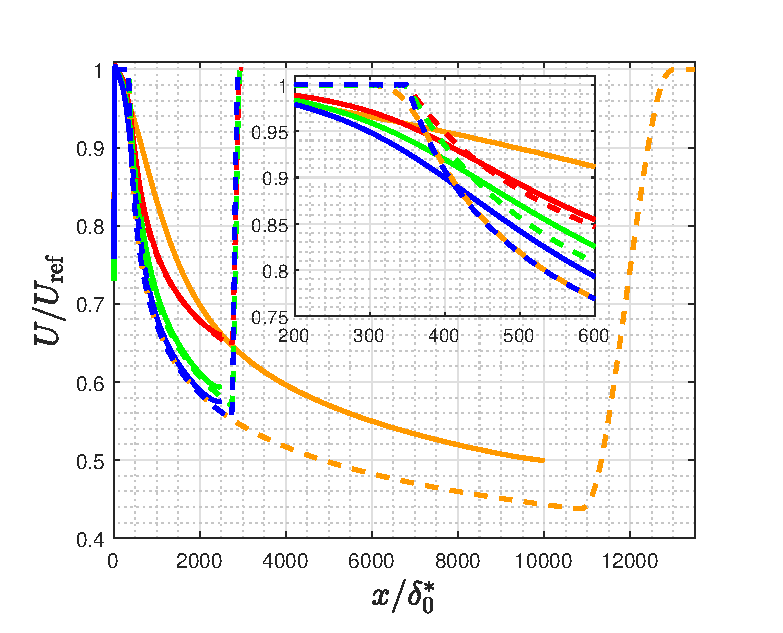
\includegraphics[width=0.6\textwidth]{fig1.eps}
  \caption{Streamwise evolution of (dashed) velocity at the top of the domain $U_{\rm top}(x)$ and (solid) velocity at the boundary-layer edge $U_e(x)$. Colors: (\protect\orangeline) b1.4; (\protect\redline) b1; (\protect\greenline) b2; (\protect\blueline) m16.}
%   Colors as in table \ref{tab:param}.}
\label{fig:U_BCs}
\end{figure}

 In figure \ref{fig:U_BCs} we show the streamwise evolution of $U_{\rm top}$ for the various cases under study, and it can be observed that this quantity is constant up to $x=350$, while it decays following a power law with different exponents $m$ for each APG \citep{bobke2017}. Note that the later rise of $U_{\rm top}$ is produced by the fringe.
 Since the BC is applied at the top of the domain and not at the edge of the BL, the velocity at the boundary-layer edge $U_e$ is not the same as $U_{\rm top}$, a fact that has been observed in multiple experiments and simulations of PG TBL and is still discussed in the scientific community as part of the problem of determining the edge of the TBL \citep{diagnostic_Vinuesa, d99_determination_2020}. The top boundary condition is far from the boundary-layer edge where the TBL  starts to develop, however, when the TBL starts to grow, this distance is reduced and the curves for $U_{\rm top}$ and $U_{e}$ come close to each other. This effect can be seen for the APGs by Bobke since the height of the domain was lower than in the larger b1.4 simulation.
 The fact that the the mean streamwise velocity $U$ exhibits a gradient ${\partial U}/{\partial y} \neq 0$ (which is a consequence of the streamwise PG) makes it harder to impose a specific velocity distribution at the edge of the BL, specially for the larger high-Reynolds simulations that require a taller computational domain for the TBL to grow. This effect could be reduced if the simulation could be performed in a domain with a variable height and not in a box of constant height.
 As a result of this effect, the imposed ZPG at $y=L_y$ is not perceived as a pure ZPG at the boundary layer edge, where the velocity instead of being constant, is slightly decaying as in an APG. As stated above, in the case where an auxiliary ZPG simulation gives the inflow, this effect of upstream influence of the APG will not be seen.
 The parameters for $U_{\rm top}$ are the same in the b1.4 and m16 cases, as can be observed in figure \ref{fig:U_BCs}, but the resulting $U_{e}$ is higher in the b1.4 than in the m16 case, which means that the decay of the velocity is not as steep in the former as in the latter and it will result in a smaller $\beta$. This shows that it is important to take into account the value of $L_y$ when setting the $U_{\rm top}(x)$ distribution to achieve a certain $U_{e}(x)$. 
 
Since we use a zero-spanwise vorticity as a BC, it is possible to rewrite the Reynolds-averaged Navier--Stokes (RANS) equations for the momentum in $x$ and $y$ in terms of the mean spanwise vorticity and its derivatives.
Being outside of the TBL means that the Reynolds stresses can be neglected if the turbulence is confined in the BL.
The first derivatives in $x$ and $y$ of $U$ and $V$ are present in the continuity equation and the mean spanwise vorticity $\Omega_z$. If those two equations are derived in $x$ and $y$ then it is possible to obtain relationships between the first derivatives of $\Omega_z$ with the second derivatives of $U$ and $V$ (present in the viscous terms of the RANS equations). Substituting the spanwise vorticity and its first derivatives in the convective and viscous terms we get:

\begin{equation}\label{eq:RANS_x_BC_OMEGA}
    U \frac {\partial U} {\partial x} + V \frac {\partial V} {\partial x} +
      \frac {1} {\rho} \frac {\partial P} {\partial x} = 
      \nu \left( \frac {\partial \Omega_z} {\partial y} \right) + V \Omega_z,
\end{equation}
\begin{equation}\label{eq:RANS_Y_BC_OMEGA}
    U \frac {\partial U} {\partial y} + V \frac {\partial V} {\partial y} +
      \frac {1} {\rho} \frac {\partial P} {\partial y} = 
      \nu \left( \frac {\partial \Omega_z} {\partial x} \right) + U \Omega_z,
\end{equation}
where $P$ is the pressure. In these equations we can see the effects of using a zero-spanwise vorticity or also making its derivatives zero. The convective terms on the left-hand side can be written as the gradient of a total pressure   $P_T / \rho = P/\rho + (U^2+V^2)/2$ caused by the effects of non-zero spanwise vorticity. Even if the spanwise vorticity is set to zero at the top of the domain, this does not guarantee that it will remain zero in all the domain outside of the TBL.
The spanwise vorticity outside of the BL is related to the curvature of $P_T$ outside of the BL due to the growth of the BL.
